\chapter{Assessment} \label{chap:assessment}

The assessment was incremental. First, the aerodynamic properties were tested on a manual flight, qualitatively, regarding properties such as stall angle, stall speed, and equilibrium point in flight. Following this, the hover capabilities were tested, such as altitude and attitude control. With the basic flight capabilities proven, a few autonomous, test flights were performed, without VTOL. Finally, its VTOL capabilities were benchmarked. These tests are better described, as well as their results, in the following sections.


\section{Tethered Attitude Control Test}

To test the attitude control and stabilization, the prototype was hang by a rope, so it's range of movement was restricted, and it was safer to test indoors.
%
The first tests were qualitative. The wing was armed on the QStabilize mode, where the gyroscope and accelerometer are used to try to maintain the aircraft leveled in VTOL mode (propellers spinning parallel to ground).
%
The expected result was that the elevons should move trying to stop the movement, even without propellers on the motors (again, for safety reasons).
%
The aircraft successfully reacted to disturbances on it's attitude by moving the control surfaces appropriately.


\section{Un-tethered Attitude Control Test} 

For this test, the wing was taken to an open field on the university.
%
For the take-off, it had to be oriented so the wind blew parallel to it's surface, so that the wind didn't flip it over.
%
Take-off cant be too slow, as the winglets adhere to the the ground and can cause the aircraft to tip over.
%
once in the air, the controls and stabilization were good, but once the wind it the aircraft, it turned it perpendicular to the direction of the wind, and the control authority was not enough for both stabilizing flight and turning the yaw axis.
%
While this problem limits the yaw controllability in VTOL mode, the position control is not necessarily affected, as the aircraft can still move in a mixed attitude between VTOL and fixed wing, inclined against the wind and maintaining position.
%

This could possibly be fixed by increasing the winglets area, however this also increases the area the wind hits, and needs more testing to verify.
%
Another possibility is tweaking the pitch angle limits, which by default are $\pm 30\degree$, in this case was not enough to fight the wind.

The flight path can be seen on Figure \ref{fig:flight1-3d}, and an in-flight photo on Figure \ref{fig:flight1-photo}. The video is available on youtube\cite{flight1}.
%
No attempt at transitioning to fixed-wing mode was made at this flight due to the reduced space available, which made the pilot feel unsafe.
	

\begin{figure}[H]
\centering
  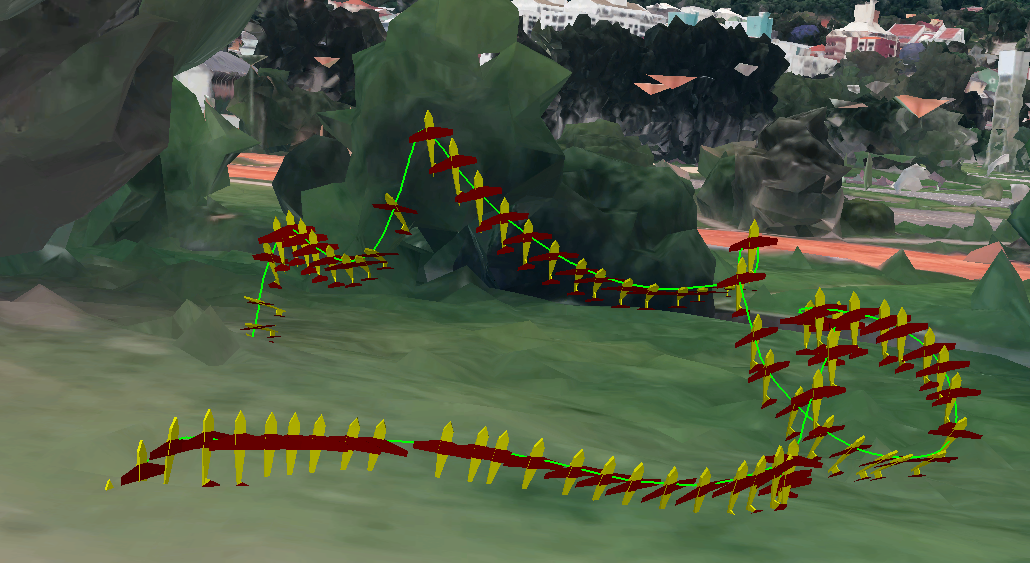
\includegraphics[width=0.7\linewidth]{figs/flight1-3d.png}
  \caption{Visualization of first test flight.}
  \label{fig:flight1-3d}
\end{figure}
	
	\begin{figure}[H]
\centering
  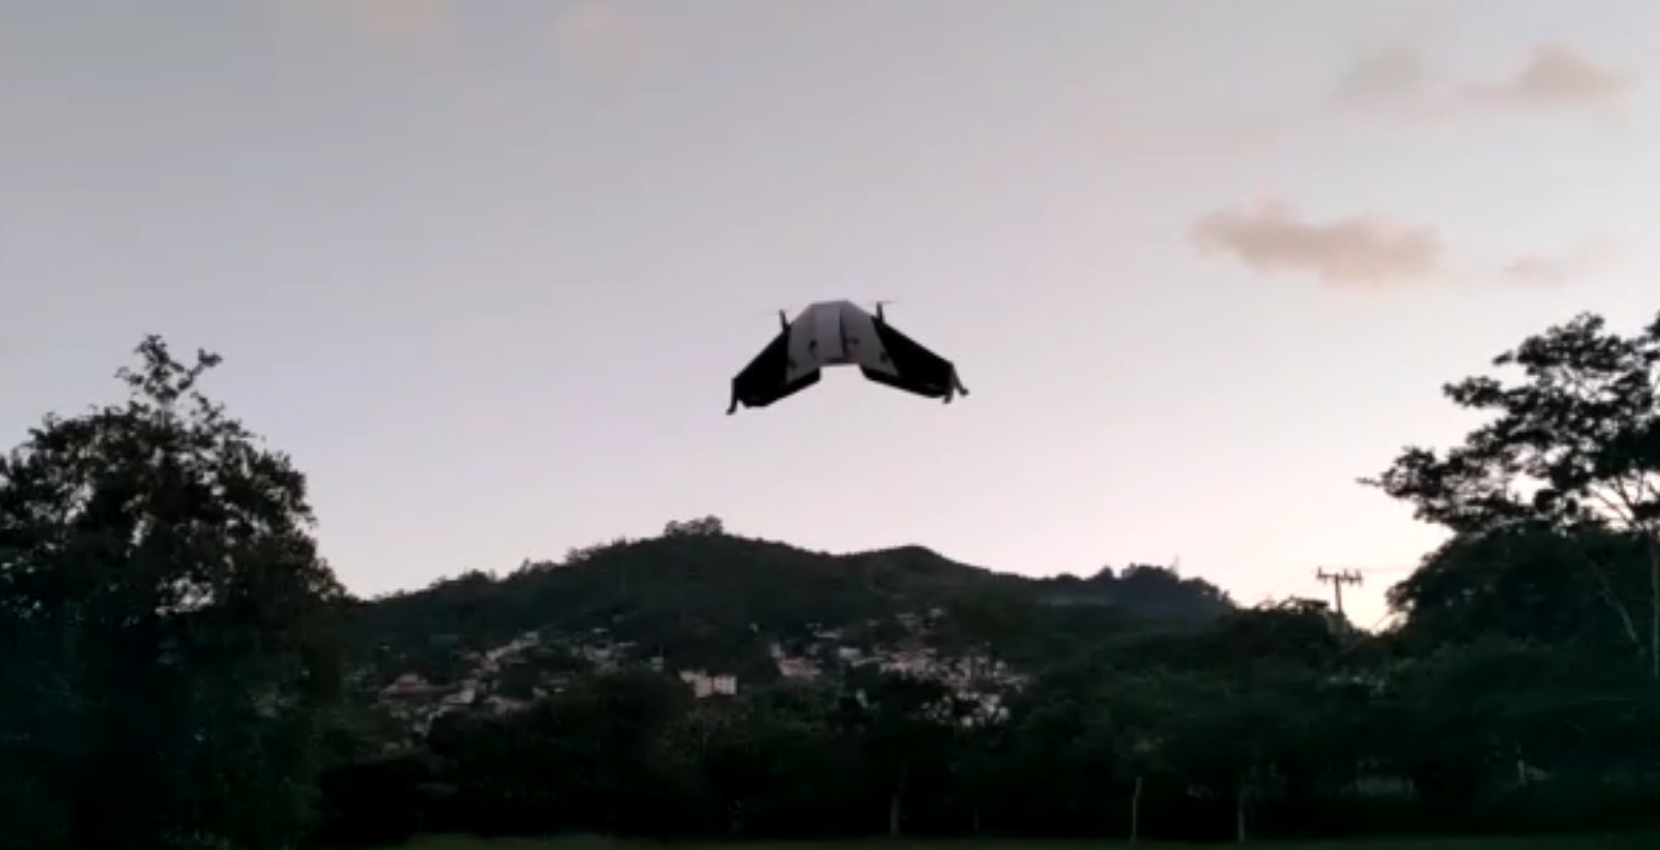
\includegraphics[width=0.7\linewidth]{figs/flight1-photo.png}
  \caption{Photo of first test flight.}
  \label{fig:flight1-photo}
\end{figure}
	



\section{Position Hold}
The next test was taking-off and landing autonomously. Due to the winds and undersized landing gear, the aircraft was positioned with the surface again parallel to the wind flow.

The autonomous take-off however, tried to take-off too slowly, and the winglet/landing gear grip to the grass limited pitch control prior to taking-off, causing the wing to tip over. The solution was to take-off manually, in QStabilize (Quadplane Stabilize) mode, then switching to QLoiter. Five of such flights were attempted. The results are on Table \ref{table:loiter}.

While most of the results were good, a roll oscillation was present on some of the flights, causing instability and forced landings.
The problem appears to be being caused by the navigation controller, as the roll("ATT.Roll") actually follows the roll setpoint("ATT.DesRoll"), who is oscillating, as seem on picture \ref{fig:rollOscillation}. This could mean that the navigation controller is oscillating fast around the given point, with increasingly high amplitude, requiring further tuning of it's parameters. 

	\begin{figure}
\centering
  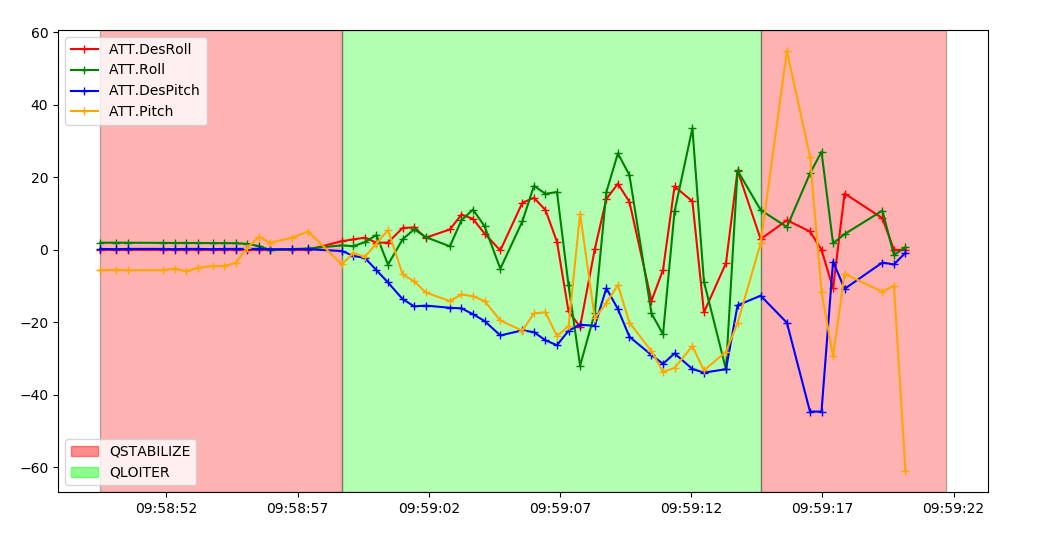
\includegraphics[width=0.9\linewidth]{figs/rolloscillation.png}
  \caption{Visualization of logged attitude control.}
  \label{fig:rollOscillation}
\end{figure}
	


\begin{table}[]
\centering

\resizebox{\textwidth}{!}{%
\begin{tabular}{@{}rrrrl@{}}

Test \# & Flight Time (s) & \begin{tabular}[c]{@{}r@{}}Position \\ Hold Radius (m)\end{tabular} & \begin{tabular}[c]{@{}r@{}}Maximum \\ Altitude (m)\end{tabular} & Notes              \\ \midrule
1       & 47              & 1.5                                                                 & 14.4                                                            &                    \\
2       & 47              & 8.1                                                                 & 12.0                                                            & Roll oscillation    \\
3       & 56              & 3.0                                                                 & 13.1                                                            &                    \\
4       & 37              & 3.7                                                                 & 4.3                                                             & Roll oscillation    \\
5       & 51              & 7.5                                                                 & 13.9                                                            & Pushed by the wind
\end{tabular}%
}
\caption{Loiter tests summary.}\label{table:loiter}
\end{table}

